\chapter{Discussion}
\label{ch:7}
In this chapter, we seek to contextualize the results from the preceding chapter. 
We apply theory from \Cref{ch:2} and compare the result to the expected behavior 
% expect from what we know about their theoretical construction/base. 

\section{Similarity Scores}

We have established that the measures define what makes trajectories similar. 
Some of the measures have a similar base idea, and thus we expect to see this reflected in the results. 
From the rankings of most similar pairs, there are a few things that stand out and we will go over them here.


%We reiterate this is not the case for all of them, and consequently, not all columns of TABLE can be used in this manner. 

First of all, EDR with $\epsilon$ set to 0.203 was the column in \Cref{tab:top-10-sim-pairs} which had the least number of frequent “most similar pairs”. 
When adjusting the parameter down to 0.101, our approximation of the recommend parameter value, all of its eight most pairs were found elsewhere in the table.
Recall that EDR’s parameter is the threshold distance that determines if points are “matching”. 
The similarity ranking with the lower parameter value aligns more with the other measures, and this could indicate that the other threshold was set too high.
We would presume that EDR would give a similar ranking as the other noise-tolerant edit-distance inspired method, MSM.
From what can be seen in the table, this appears to hold, but it varies with its parameter value too. 

%   that would have similar values to the

Next, we note that the Hausdorff distance generated similar pairs which were quite different from the other measures. 
As the Hausdorff metric is parameter-free, we reckon that the reason its results stood out was that it defined trajectory similarity in a different manner than the rest. 
We established that the Hausdorff distance does not take into account the direction of a trajectory and the only other measure that is invariant to direction is SSPD. 
Indeed they share many of the top 10 ranked scores, however, SSPD distinguishes itself Hd as it reduces the similarity score to a single element-element pair making altering their internal rankings again. 

% Next we observe that the Hausdorff distance contains the second least “frequent pairs” and as it parameter free, we reason that there must be something with how it defines trajectory similarity that makes it stand out. Recall that the Hausdorff distance stood out as the only measure that did not take into account the direction of a trajectory. Furthermore, it stands out as the only measure that reduces the similarity distance to an element-element pair.

The final observation from \Cref{tab:top-10-sim-pairs} we noted was that Euclidean distance, ERP, and one of the MSM measures gave the exact same top 10 pairs. 
Upon closer examination, it turned out that their ranking remained the same until the 44th pair, and the similitude between the measures continued beyond that.
MSM with cost value 1 and the Euclidean distance's ranking match for 9456 of the 10 thousand most similar trajectory pairs. 
We reason that this occurred as a consequence of the cost of Splits and Merges being set too high, making MSM  default to the Move operation whose cost is the $L_2$ norm between trajectory elements.
As for ERP, we reason that setting the reference point, $g$, to the origin, increased the cost for trajectory elements that were far away.
Again, making the method depend on the $L_2$ norm between trajectory elements as the cost of an edit.


\section{Davies-Bouldin Results}

The essence of this thesis is to examine how the definition of similarity varies with different measures.
Clustering is a manner of grouping the trajectories such that traits which are seen as the most defining characteristics under various definitions get highlighted. 

As stated in \Cref{ch:2}, there are a number of cluster evaluation techniques that aim to numerically rank the quality of clustering results.
One of these is the DB-index however we will not an assumption regarding which type of type similarity was the most “correct” one.
The ranking created by this criterion is not invalid, but the insight it adds to is limited.
Nevertheless, we have chosen to leave in this stage of the experiment and in the report on the account of the efforts that were put into computing it as well as its natural role as a starting point for analyzing the clusters. 
 
Our version of Davis-Bouldin favors clusterings where each trajectory element differs as little as possible from the mean of all trajectory elements when computed in a. A consequence of this is that the cluster can appear fuzzy since the placement of the surrounding points does not affect the index. 
From \Cref{tab:cluster-dbidx} it appears as if the lock-step method and EDR with threshold parameter $\epsilon=0.203$ were the best performing methods, and this is as expected. 

Moreover, methods that do not take into account order observations, or methods that would reorder the trajectory elements received low DB-index rankings. In \Cref{fig:cluster-best-worst-db-ap,fig:cluster-best-worst-db-h}  the clusters that were generated by the measures which received highest and lowest DB-indexes are drawn. These figures illustrate the bias of our DB-index implementation. 


\begin{figure}[h!]
  \centering
  \hspace{1em}
   \begin{subfigure}[c]{0.37\linewidth}
     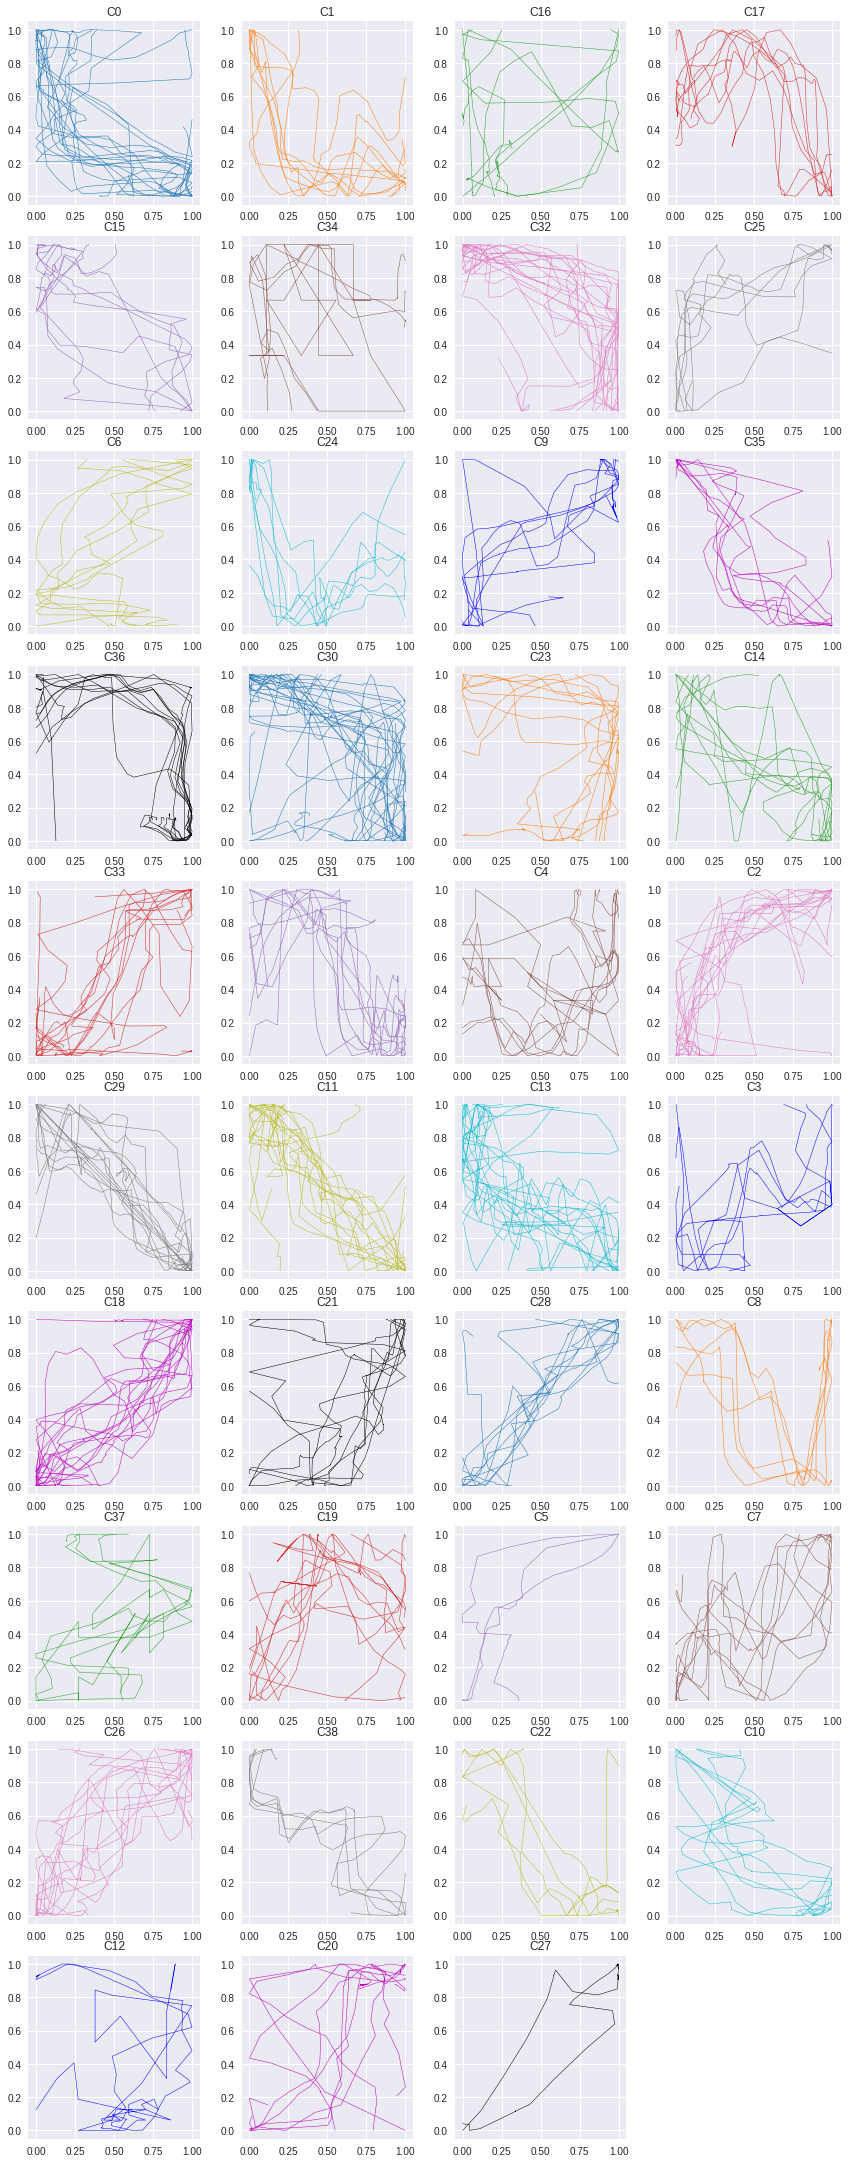
\includegraphics[width=\linewidth]{figs/clusters/CLU_AP_ALL[EDR;e=.203].png}
    \caption{EDR;$\epsilon=0.203$, highest rank}
  \end{subfigure}
  \hfill
  \begin{subfigure}[c]{0.37\linewidth}
    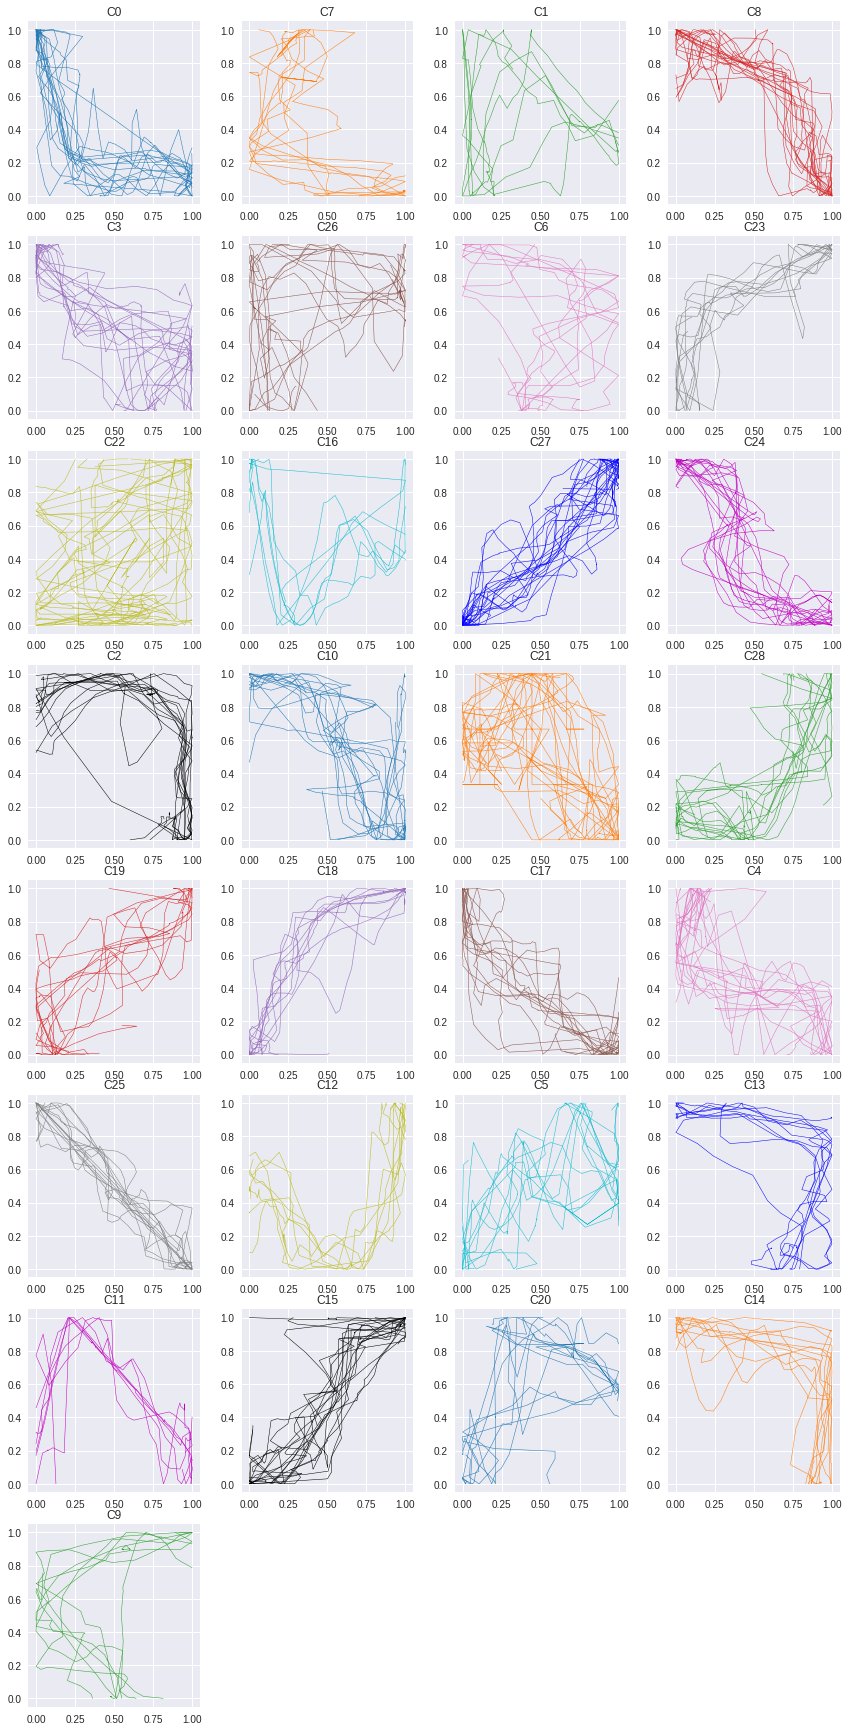
\includegraphics[width=\linewidth]{figs/clusters/CLU_AP_ALL[SSPD].png}
    \caption{SSPD, lowest rank}
  \end{subfigure}
  \caption{The AP-clusters of the measures the best and wort Davies-Bouldin indexes.}
  \label{fig:cluster-best-worst-db-ap}
\end{figure}

\begin{figure}[h!]
  \centering
  \hspace{1em}
   \begin{subfigure}[c]{0.4\linewidth}
     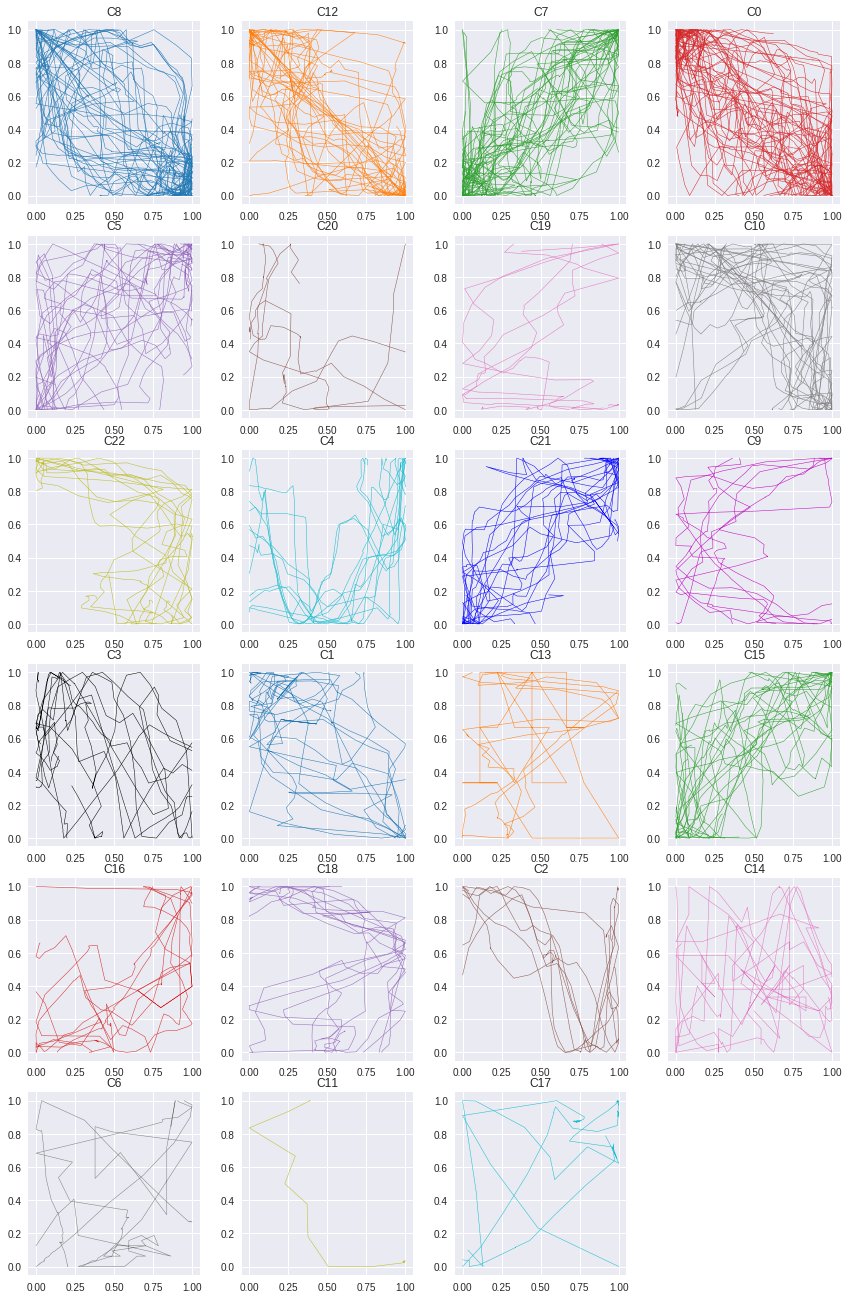
\includegraphics[width=\linewidth]{figs/clusters/CLU_H_ALL[ERP;g=0,0].png}
    \caption{ERP, $\epsilon=0.203$, highest rank}
  \end{subfigure}
  \hfill
  \begin{subfigure}[c]{0.4\linewidth}
    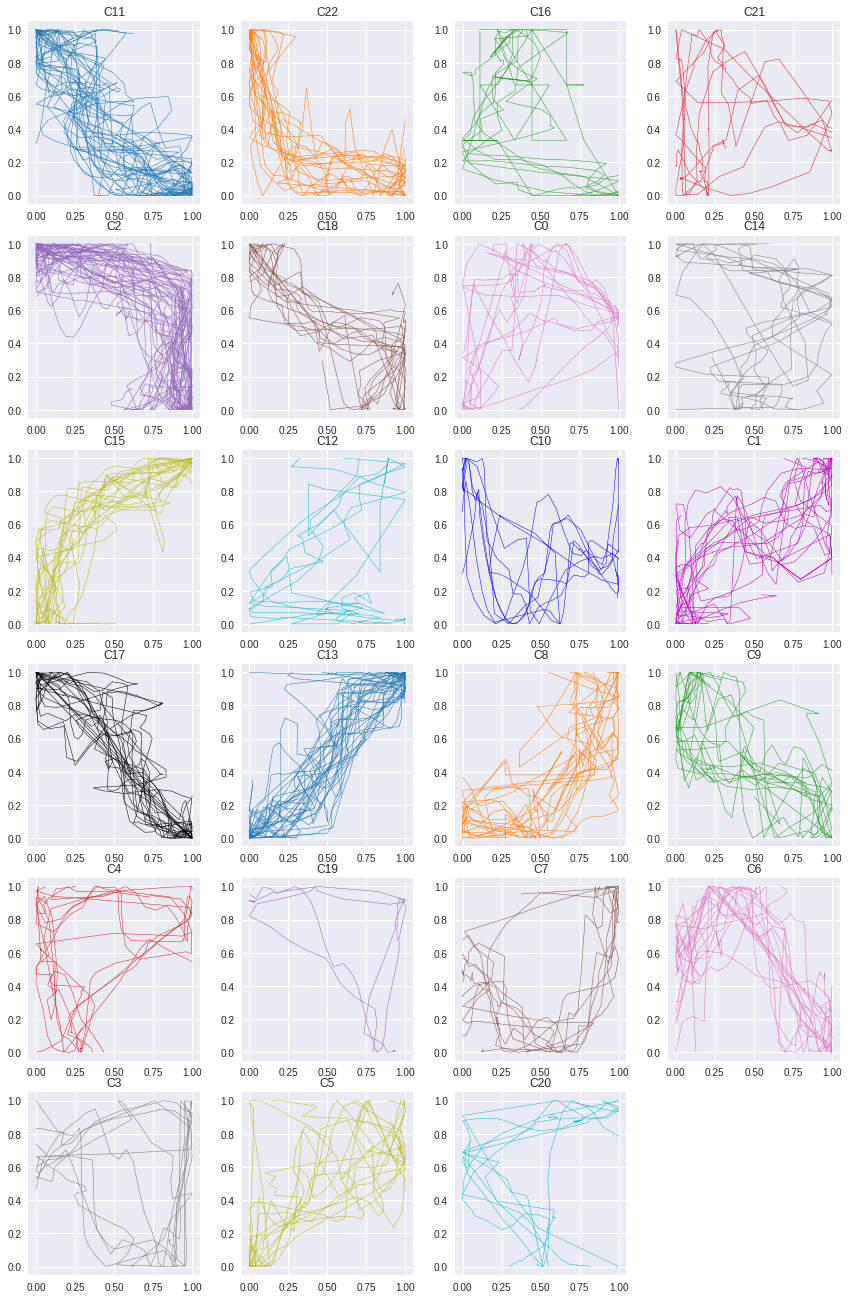
\includegraphics[width=\linewidth]{figs/clusters/CLU_H_ALL[SSPD].png}
    \caption{SSPD, lowest rank}
  \end{subfigure}
  \caption{The HCA-clusters of the measures the best and wort Davies-Bouldin indexes.}
  \label{fig:cluster-best-worst-db-h}
\end{figure}



As a consequence of the unreliability of the DB-index, the main tool for examining the clusters will be visual inspection.
This will allow us to account for the different aspects of trajectory similarity and formulate conclusions accordingly. 
Re-examining \Cref{fig:cluster-best-worst-db-ap,fig:cluster-best-worst-db-h} with visual inspection it would appear that SSPD produced cleaner and fewer clusters than both EDR and ERP. 
This is in stark contrast to the ranking created by the Davies-Bouldin criteria under both HCA and AP analysis. 


This evaluation alternative comes with its own drawbacks, one of which is the matter of subjectivity. 
At the same time, it has been stated that human assessment is an important component for determining the quality of clusters\cite{79-SilhouetteAnalysis}. 
We will not be declaring any measure better than the others as our results do not provide support for an accurate ranking.



% We cannot declare one measure just better than all others from the evaluation that we executed here as it makes no sense. This is in large part due to the inherent bias of using a strict lockstep method to evaluate the final clusters. 
% By visual inspection, SSPD produced cleaner and fewer clusters than EDR, $\epsilon=0.203$ under AP, despite having a much worse criterion. This pattern repeats itself under HCA when predetermined even with  the amount of final clusters. EDR  as well \Cref{fig:cluster-best-worst-h-db}.

% Based on those arguments, the main tool for examining the clusters will be visual inspection. This will allow us to account for the different definitions/aspects of similarity and formulate conclusions in an aggregate manner. 
% This method comes with its own drawbacks, one of which is the matter of subjectivity. Yet as brought up in supported previous works[CITATIONS], human assessment key for determining the quality of clusters. 




\section{Cluster Behavior}

First, we describe what we expected the clusters to look like based on the properties of the specific similarly distance function. 
For the methods that operate with a parameter value, we discuss how changing that value would affect the cluster results.
Then we compare our expectations to the clusters themselves.
Affinity propagation is a was the parameter-free method, thus its results are weighted more.
On the other hand, the number of hierarchical clusters was arbitrarily set, leading us to use its results as a supplementary evaluation. 


% https://www.wordhippo.com/what-is/another-word-for/foreseeable.html 
\subsection{Expectations}
In general, there are three factors that will affect how we expect the final clusters to appear. 
Measures that are context-aware should calculate fewer fuzzy clusters.  
Next, measures that account for local time shifts should group trajectories that have similar sub-sections but with an offset creating a wider band of similarity.
Lastly, we expect the noise-sensitive trajectories to create fuzzier trajectories.  


\textbf{Euclidean Distance} is the only lock-step measure, and trajectories that are in the same region might receive an artificially high similarly score by nature of being near each other. 
A trajectory pair will be rewarded if they have elements at the same index which are near each.
This would create fuzzy clusters as each point evaluated isolation and taking the average of the pairwise element-distances will artificially smooth out the distances.
An extra amount of fuzziness is expected to come from the fact that this measure is sensitive to noise. 

% WE COULD observe that there are trajectories that oscillate around the same region at a similar pace- giving them a lock-step similar score, but the cluster ends up looking fuzzy. 

\clearpage
\textbf{Dynamic Time Warping}  optimizes for local shape similarity and warps trajectories to reflect similarity after shape-preserving transformations.
We expect the final clusters to appear fuzzy at first glance as the local similarities would be out of sync. 
Yet upon closer examination, we should be able to spot bands of cohesive trajectory sections. 
DTW is a noise-sensitive method, so we would expect some level of fuzziness to be present, however, the clusters should be crisper than that of the Ed. 



From \textbf{Hausdorff Distance}, we would expect crisper clusters than both Ed and DTW if we could guarantee the data free of noise.
The maximizing over a minimum of all element-element pairings means that the overall shape similarity is weighted in a way that the other measures do not account for. 
In other words, the global resemblance matters more under this definition. 
However, the data set we used is not noise-free so while we expect some crispness, there will be fuzziness of the clusters due to its noise sensitivity.

% All of the trajectories' points have to be near each other for if the pair is to receive a high similarity score.
% stemming from the reduction of similarity distance to distance between two trajectory elements. 

One of the key features of \textbf{Symmetrized Segment-Path Distance} is that it accounts for whole trajectory shape similarity. 
This means that we expect it to generate the crispest looking clusters. 
The expectation of crisp clusters is further substantiated by its tolerance to noise
This method aimed to be invariant to the physical locations, meaning that trajectories of similar shapes with different origins could be grouped together. This could result in some broader bands of similarity.

% All of the parametric measures adapt to local time shifts like in the same manner as DTW, and  therefore we expect the clusters they generate exhibit some of the same type of fuzziness. This, of course, is not the only factor that affects how fuzzy or crisp the clusters become. The choice of parameter, as well as the (internal workings) of the algorithms matter greatly.  
%SOMETHING ABOUT HOW DTW ERP etc have re-s sim to dtw as noted in \cite{26}


Recall that \textbf{Edit Distance on Real Sequences} uses the parameter $\epsilon$ to as the matching threshold for how close how two trajectory elements are.
Decreasing the parameter value leads to an increase in strictness in how close elements have to be, and in turn, would lead to crisper clusters.
It goes without saying that a too restrictive $\epsilon$ would no longer be accurate; if no trajectory elements are matching, the only basis for similarity would be the trajectory lengths. 
Clusters are expected to have some level of fuzziness as EDR considers the trajectory element in isolation. 


\textbf{Edit Distance with Real Penalty} was computed with one parameter value.
We have established that this metric is sensitive to noise and that it accommodates local time shifts.
As EDR, this measure does isolates the trajectory elements when computing the similarity distance. 
This means that there are three factors that contribute to fuzzy clusters, thus we expect the fuzziest clusters to be generated from this metric.  
% As it is a measure that handles local time shifts and does not compare a trajectory as a whole, we expect the clusters to appear quite fuzzy. This expectation is further supported by its low tolerance to noise. 


\textbf{Move-Split-Merge} handles local time shifts in the same manner as DTW and the other Edit Distance-based measures.
We expect to observe trajectory sections that match and create wider bands. 
MSM distinguishes itself by accounting for the values that surround a given element when computing the similarity score. 
This means that we expect the clusters are crisper than those of generated by EDR and ERP. 
The parameter of MSM determines to which degree Splits and Merges are favored over Moves. 
As the cost increases, they will increasingly be evaded in favor of directly substituting the element. 
The cost of a Move is pairwise element-element distance, and in turn, the clusters would resemble those created by a Euclidean distance based measure. 
On the other hand, if the parameter is set too low we expect more trajectories that do not resemble each other to get clustered together. 


%I thin,, it is hard to tell

% Finally we study how we expect the change of the cost of MSM transformations to impact the final clusters. The parameter determines how much splits and merges should be favored over moves. At the extreme end, MSM will resemble DTW as element-element distance would dominate the cost matrix. That is, the higher the value of c, the more the cluster should resemble DTW. For lower values of c, we should see a preference for actively splitting and merging, bringing its cluster results closer to that of ERP. 

% Setting the cost to 1, results in similarity scores that are


\subsection{Visual Inspection}

The visual inspection inspects the apparent fuzziness of the clusters as well as how scatted the trajectories within a cluster are. 
We will refer to the latter of these characteristics as the \textit{band} of similarity which describes the general \textit{trend} of the cluster. 
Where is it possible, we remark how larger trajectory sections were processed. 
Unfortunately, spotting tendencies like that is not something visual inspection excels at.

In the case of affinity propagation, we take note of how many clusters it generated. 
The corresponding evaluation for the hierarchical clusters is taking note of how balanced the final clusters are.
With how hierarchical clusters are created, some imbalance is expected as the most distinct trajectories will be connected last.

% contour  
%  silhouette
%  hierarchical affinity

\textbf{Euclidean Distance:}
\begin{itemize}
\item AP:  In terms of overall shape, the clusters appear very fuzzy. 
There are some clusters where that have a clearer contour and some where it is possible to spot a trend for the trajectories. 
Nevertheless the general impression remains fuzzy; we observe trajectories that seem to oscillate freely around the apparent trajectory band.
While oscillations make the clusters appear fuzzier, the clusters do not come across as randomly grouped observations. 

\medskip
\item HCA: There appears to be a bias and clusters are unbalanced. 
Some of the clusters contained a few trajectories while some of them encompassed a large number of them.
In those clusters the bands were obvious, but the oscillations were even greater than those observed under AP.
This makes sense as the new clusters are created by merging similar sub-clusters. 
We would expect a clearer band, but a fuzzier contour. 
\end{itemize}

\textbf{Dynamic Time Warping:}
\begin{itemize}
\item AP: We observed two clusters that were very crisp and even more clusters that exhibited clear trends. 
The trajectories do not seem to oscillate around the band in the clusters as much as they did under Ed. 
We can spot some trajectory sections that appear as if they have been re-aligned– leading to a less messy expression. 
Still, there are some oscillations and noisy clusters that make it hard to tell exactly why some trajectories were clustered together. 
\medskip  
\clearpage
\item HCA: The clusters are unbalanced, however less so than the ones created by Ed. 
They illustrate how shape similarity is persevered under this measure by displaying a clear trend in the clusters. 
Yet, the clusters are fuzzy in that their trajectories still deviate from the central band. 
From these clusters it appears as if some of the trajectories are outliers; 
they appear to be distinct from the rest of the trajectories and are placed in their own clusters. 
\end{itemize}


\textbf{Hausdorff Distance}
\begin{itemize}

\item AP: Compared to DTW and Ed, the final number of clusters increased and the clusters created were both crisper and fuzzier. 
The clusters display both the most advantageous and most disadvantageous aspects of the Hausdorff metric. 
% Reducing the similarity score to one element-element distance did indeed  amount
However, the number of crisp clusters outweighs the fuzzy ones, and the contours of the clusters are crisp enough to highlight more intricate trajectory details. 
% This contrasts the other clusters clustered together, rather than a general direction across the grid

\medskip
\item HCA: Again, we see both crisp and intricate clusters as well as very fuzzy ones. 
The observations from affinity propagation hold for these clusters as well; 
both the advantages and disadvantages of setting the similarity score as the distance between two trajectory elements are highlighted. 
There is one cluster that is so fussy that we were quite puzzled by how it was formed.
% It may be that trajectories with outliers and noise were put together in such a way that they were at some point considered so similar to each other that they were gathered. 
\end{itemize}


\textbf{Symmetrized Segment-Path Distance:}
\begin{itemize}

\item AP: This measure created fewer clusters than Hd, yet the clusters it created appear to be at least equally as crisp.
We observed that the clusters had such tight bands that curves of the trajectories were accentuated.
In contrast, DTW clustered the trajectories by their general shape and direction.
Whereas Hd was sensitive to noise, it becomes clear that SSPD addressed that weakness.
Two clusters stand out as more fuzzy than the others, but this is likely due to noisy data.
\medskip 
\item HCA: The clusters are about as balanced as those created by Hd. 
As was demonstrated in the AP-clustering, there is a trend towards showing the intricacies of shape similarity at a larger scale. 
The bands of similarity are thinner than both Ed end DTW and more detailed than Hd. 
\end{itemize}


\textbf{Edit Distance with Real Penalty:}
\begin{itemize}

\item AP:  The clusters created by ERP are significantly more fuzzy than that of Hd and SSPD. 
This is expected as it gives similarity scores based on edits before and then the distance between trajectory elements.
However, it is unexpected that the resulting clusters were as fuzzy as those created by DTW and Ed, especially as it created far more clusters than either of them did.
The increased number of clusters should indicate that we would have more distinguished clusters, but this does not appear to be the case.
Even still, we observe that clusters were not randomly put together.
Looking closer at specific clusters, it is possible to spot turns and segments that are just shifted from each other. 
\medskip
\item HCA: These clusters are unbalanced, there is a cluster that only has one trajectory. 
Yet, that trajectory does not appear significantly distinct from the ones existing clusters. 
From visual inspection it challenging to get more insight. 
The bands across the clusters are quite general and there is not a consistent show of shifted segments.

\end{itemize}

\textbf{Edit Distance on Real Sequence: }
In discussing this method, we examine the clusters obtained from both parameter values in parallel.  
% $\epsilon = \{0.101, 0.201\}$


% contour  
%  silhouette
%  hierarchical affinity propagation

\begin{itemize}
\item AP: This measure generated the two largest number of AP-clusters. 
The most restrictive parameter led to 48 clusters while the other value resulted in 39 clusters. 
In our subjective opinion, both of the parameters resulted in too many clusters for a data set of 300 observations. 
However, with fewer trajectories in each cluster analysis through visual inspection becomes is easier.
We observed that the clusters contained trajectories whose segments were shifted from each other. 
Both parameter values resulted in crisp clusters, and our approximation of the recommended value gave seemingly more defined contours. 
While increasing the threshold value led to fuzzier clusters, these clusters were crisper than those of ERP. 
This is an expected result as EDR is noise-tolerant whereas ERP is not.
\medskip  
\item HCA: For both parameter values, there were bands that obscured the intricacies of shape similarity.
Once more we observed that increasing the parameter value resulted in fuzzier clusters. 
However, the increase in fuzziness was less than expected. 
The largest parameter value led to a more unbalanced distribution of trajectories, further signifying that the smaller one remains the most suited value for $\epsilon$.
\end{itemize}


\textbf{Move-Split-Merge:}

As we did for EDR, the clusters created by MSM and the effect of varying the parameter are discussed in parallel. 
We first note that the clusters MSM created with the cost was set to 1 and were indistinguishable from those of Ed. 
This was not an entirely unexpected result given what we know about MSM, and that the two methods had identical rankings of the most similar trajectory pairs. 
By reason of that cost parameter being set too high and the accompanying clusters already being described, we will focus on the two remaining parameter values. 

  % cost$= \{1, 0.1, 0.01\}$
\begin{itemize}

\item AP: We observed that the lowest parameter value resulted in fewer clusters, but both of the parameter values led to a larger number of clusters than expected.
As with EDR, the large number of clusters makes it easier to visually analyze them. 
Given that this measure is both moderately noise-tolerant and context-aware we expect the clusters to be crisp.
Indeed, the majority of the clusters have crisp contours wherein the intricacies of the trajectories are preserved.
Some clusters contain what appear to be outlier trajectories.
This would suggest that the discrimination degree of this measure was high enough to isolate them in a way that no measures did. 
The smaller parameter value resulted in both fuzzier clusters and an increase in clusters with few trajectories.
This may be an indication of that value being too low, suggesting that $0.1$ was the most appropriate cost for this data set. 

\medskip  
\item HCA: The clusters created by the lowest cost parameter were more unbalanced and fuzzier than those generated by the middle one. 
This further supports the argument that the middle of the cost value is the most fitting one. 
Interestingly, there were still trajectories that were clustered by themselves as if they were outliers. 
It looks as if these trajectories are consistent across both parameter values and clustering techniques. 

\end{itemize}





\section{Reflections}
% Other Applications write here, but i i think it might belong to "further work"

The measures created clusters whose qualities coincide with the anticipated results. 
We observed fuzzy clusters where the underlying measure was less tolerant to noise and crisper clusters where the measure accounted for whole trajectory similarity.
Almost all of the measures were elastic, and we observed several clusters with trajectories that were time-shifted. 

By visual inspection, it was hard to tell if metricity affected the clusters although this may have been a result of picking clustering techniques that did not require a metric distance function. 
% metricity. 

The clusters' appearance remained consistent between AP and HCA for a given measure, even as the number of clusters changed. 
This observation was to be expected as the models that created the clusters used the same similarity distances scores. 

Lastly, we comment on a few algorithm-specific observations. 
The fuzziness of the clusters created by the Euclidean distance align with its lock-step design just as the crispness of SSPD’s clusters aligns with its design purposes. 
It was initially unexpected that ERP would have the fuzziest looking clusters. However, upon closer examination, we reasoned that it made sense that a non-context aware, noise sensitive method that adapts to time shifts would lead to quite fuzzy clusters. 

The way MSM could consistently filter out trajectories that did not behave like the others would imply that it would be well suited for outlier detection. 

% For \textbf{MSM} the effects of its parameter, setting $c$ to $0.1$ resulted in AP generating a cluster consisting of just one trajectory and decreasing it $0.01$  lead to 5 of these single trajectory clusters. This could be an indication of poorly chosen parameter values. Looking at the HCA- generated clusters support this assumption. We observed less balanced clusters as the cost parameter decreased. Based on this, we have conclude that MSM with cost parameter $c=1$ best is the most representative for this measure and further analysis will be based on it.  



\section{Inconsistencies from Simplifications}
As noted in \Cref{ch:5}, several simplifications were made for this experiment.
We close this chapter by reflecting on how these simplifications have affected the results.

% \clearpage

\subsection{Data format}
%  For real life data, it is not reasonable to assume that the trajectories will be of the same length and furthermore, if the trajectories are of the same length this still does not mean the time spent in each location matches up.

The first simplification that was made was truncating the trajectories to equal length.
In doing this we removed the option to study how measures would have handled cases like this.
There would be insight to be gained from examining measures at different trajectory lengths. 
In particular, it is not reasonable to assume that real data would have this property. 
The clusters could have ended up looking quite different, possibly highlighting the difference between trajectory section and whole trajectory similarity.

Of the algorithms in this thesis, only the Euclidean distance lacked a definition for trajectories of unequal length. 
It is possible to design a comparative study where lock-step measures can give scores for these trajectories. 
An option would be to artificially add more trajectories elements by interpolation. 
However, we decided against it as we felt confident there would be enough properties to examine after the simplification. 

The next data-format simplification we did was the re-scaling.
The manner in which it was done meant that the data would lose its connection to the real world.
To exemplify this we refer to \Cref{fig:sspd_loc_real}. 
The clusters were created based on the scaled data, thus those clustered were quite crisp. 
However, when displaying those same clusters with their raw coordinates it becomes clear how scattered the trajectories are.
It becomes clearer that trajectories were clustered together based on shape similarity. 
We reiterate that the intent was to study measures themselves, thus the data set selection— and thereby the re-scaling was inconsequential. 



\begin{figure}[h]
  \centering
  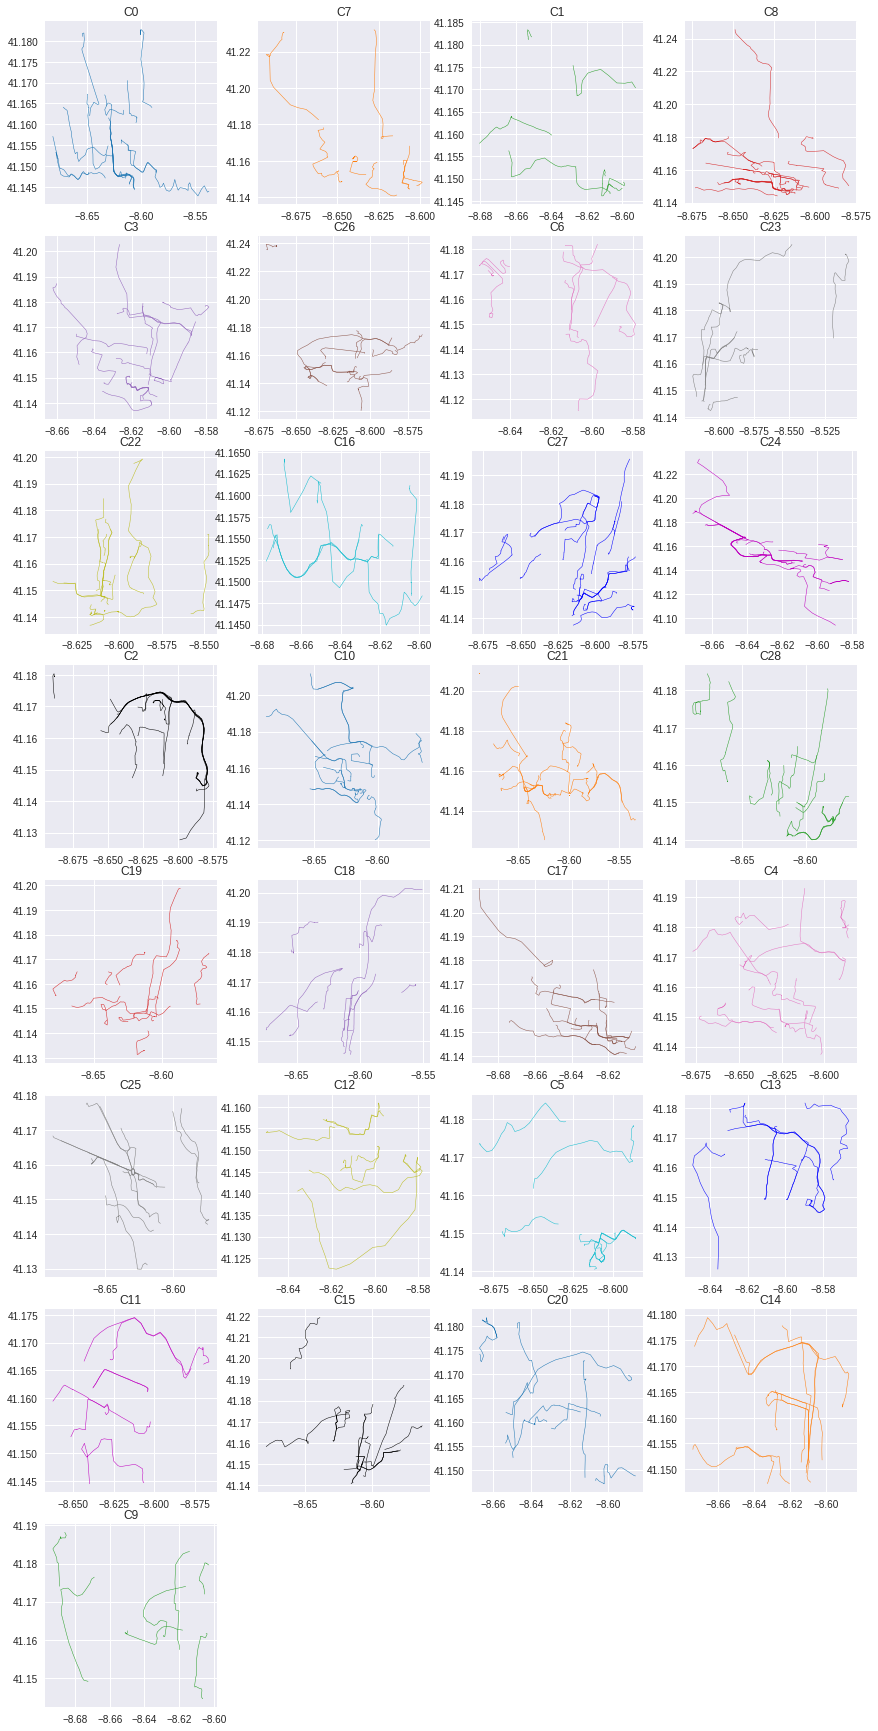
\includegraphics[width=.9\linewidth,height=.9\textheight,keepaspectratio]{figs/clusters/CLU_AP_ALL[SSPD]_REAL.png}
  \caption{Affinity propagation clusters created with SSPD, but showing the raw trajectory locations}
  \label{fig:sspd_loc_real}
\end{figure}


\subsection{Distance Computation and Evaluation}
% Tweaking the format and scale of the data is one thing, but the next line of simplifications mattered more for the evaluations of the measures. 

We tested three measures that required a parameter and we did not do any proper parameter tuning. 
ERP would likely have had more agreement with the other measures in \Cref{tab:top-10-sim-pairs} if different values for the reference point had been tested out. 


% Next, while we did not  the measues 

% The last simplification we would like to bring attention to is also something that potentially affected the final evaluation. 

The application we chose for the similarity distance measures, clustering, is itself an area of active research. 
The interconnectedness of clustering techniques and distance algorithms could have been studied in more detail before settling on affinity propagation and hierarchical clustering analysis as the evaluation basis.
We acknowledge that there may be traits of the selected measures that have been obscured or misrepresented. 

